
% Large version
% \begin{tikzpicture}[scale=.5]
% %\def\bndmax{5}        %https://tex.stackexchange.com/questions/68462/filling-a-complex-region-with-tikz
% %\def\bndmin{0.2}
% \def \Y {10}  % height of y axis pecent
% \def \W {20}  % length  of x axis
% \def \Wbar {3} % jmeam wealth
% \def \omega {3}
% \def \A {1}  %was .5
% \def \B {.5}
% %Equation   \[ r_i = (A + .5 \frac{\bar{W}}{W_i})\omega\]
% \def \Wmin{.63}  %This sets the lower limit fo the 
% \def \Wmin{(\B*\Wbar)/(\Y/\omega-\A)} %function to keep in in bounds
	
% \tikzset{func/.style={thick,color=blue!90}}	

% \draw [thick] (0,\Y)node[left=.5cm]{$r_i$} -- (0,0)--(\W,0)node[below]{Wealth};  	% Axes
% \draw [thick] (0,\omega)node[left=.5cm]{$\bar r$} -- (\W,\omega);  	% Axes
% \draw [thick,dashed] ( \Wbar,0)node[below=.5cm]{$\bar{W}$} -- (\Wbar,\Y);  	% Axes

% \foreach \yi in {0,...,\Y} \draw (0,\yi)--(-.1,\yi)node[left]{\small$\yi$};

% \draw[func,domain=\Wmin:\W] plot [samples=200] (\x,{(\A+\B*\Wbar/\x)*\omega});
% \def \A {.8}
% \draw[func,domain=\Wmin:\W, green] plot [samples=200] (\x,{(\A+\B*\Wbar/\x)*\omega});

% \def \A {1}
% \def \B {.8}
% \draw[func,domain=\Wmin:\W, red] plot [samples=200] (\x,{(\A+\B*\Wbar/\x)*\omega});

% \draw [red,  thick](13, 9)--(15,9)node [right, black] {\small A=\ 1,\ B=0.8};
% \draw [blue,  thick](13, 8.3)--(15,8.3)node [right, black] {\small A=\ 1,\ B=0.5};
% \draw [green, thick](13, 7.6)--(15,7.6)node [right, black] {\small A=.8, B=0.8};
% \end{tikzpicture}


\[   r^h=\frac{ \delta(1+\dot p  - (1+r)m) \ + \rho   	-\kappa - t } {1-m}    \]
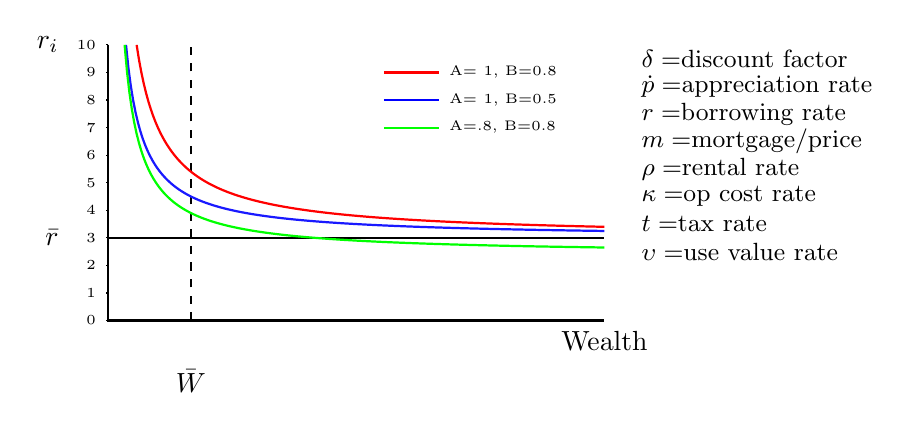
\begin{tikzpicture}[scale=.35]
%\def\bndmax{5}        %https://tex.stackexchange.com/questions/68462/filling-a-complex-region-with-tikz
%\def\bndmin{0.2}
\def \Y {10}  % height of y axis percent
\def \W {18}  % length  of x axis
\def \Wbar {3} % j mean wealth
\def \omega {3}
\def \A {1}  %was .5
\def \B {.5}
%Equation   \[ r_i = (A + .5 \frac{\bar{W}}{W_i})\omega\]
\def \Wmin{.63}  %This sets the lower limit fo the 
\def \Wmin{(\B*\Wbar)/(\Y/\omega-\A)} %function to keep in in bounds
	
\tikzset{func/.style={thick,color=blue!90}}	

\draw [thick] (0,\Y)node[left=.5cm]{$r_i$} -- (0,0)--(\W,0)node[below]{Wealth};  	% Axes
\draw [thick] (0,\omega)node[left=.5cm]{$\bar r$} -- (\W,\omega);  	% Axes
\draw [thick,dashed] ( \Wbar,0)node[below=.5cm]{$\bar{W}$} -- (\Wbar,\Y);  	% Axes

\foreach \yi in {0,...,\Y} \draw (0,\yi)--(-.1,\yi)node[left]{\tiny$\yi$};

\draw[func,domain=\Wmin:\W] plot [samples=200] (\x,{(\A+\B*\Wbar/\x)*\omega});
\def \A {.8}
\draw[func,domain=\Wmin:\W, green] plot [samples=200] (\x,{(\A+\B*\Wbar/\x)*\omega});

\def \A {1}
\def \B {.8}
\draw[func,domain=\Wmin:\W, red] plot [samples=200] (\x,{(\A+\B*\Wbar/\x)*\omega});

\draw [red,  thick](10, 9)--(12,9)node [right, black] {\tiny A=\ 1,\ B=0.8};
\draw [blue,  thick](10, 8)--(12,8)node [right, black] {\tiny A=\ 1,\ B=0.5};
\draw [green, thick](10, 7)--(12,7)node [right, black] {\tiny A=.8, B=0.8};

\def \W {19}  % length  of x axis
\node[right] at (\W,9.5){\small$\delta=$discount factor};
\node[right] at (\W,8.5){\small$\dot p=$appreciation rate};
\node[right] at (\W,7.5){\small$r=$borrowing rate};
\node[right] at (\W,6.5){\small$m=$mortgage/price};
\node[right] at (\W,5.5){\small$\rho=$rental  rate};
\node[right] at (\W,4.5){\small$\kappa=$op cost rate};
\node[right] at (\W,3.5){\small$t=$tax rate};
\node[right] at (\W,2.5){\small$\upsilon=$use value rate};
 \end{tikzpicture}

